\documentclass{article}

\usepackage{lipsum}
\usepackage[margin=2cm, left=2cm, includefoot]{geometry}
\usepackage{graphicx}
\usepackage{float}
\usepackage{hyperref}

% Header and footer
\usepackage{fancyhdr}
\pagestyle{fancy}

\rhead{}
\lhead{}
\fancyfoot{}
\fancyfoot[R]{\thepage}
\renewcommand{\headrulewidth}{0pt}
\renewcommand{\footrulewidth}{0pt}
%

\begin{document}

\begin{titlepage}
	\begin{center}
		\line(1,0){300}\\
		[6mm]
		\huge{\bfseries PROJECT TENDER}\\
		[2mm]
		\line(1,0){200}\\
		[5mm]
		\large\textbf{PROJECT:}\\\textsc{Network Visualizations Interface for Large Scale Networks}\\
		[3mm]
		\large\textbf{CLIENT:}\\\textsc{Ivan du Toit}\\
		[3mm]
		\large \textbf{TEAM:}\\\textsc{Funge}\\
		\line(1,0){350}\\
		[5mm]
		\large \textbf{Team Members:}\\
		[3mm]
		\large Gian Paolo Buffo - 14446619\\
		\large Matthew Botha - 14214742\\
		\large Matthias Harvey - 14027021\\
        \large Dillon Heins - 14035538\\[3mm]
		\begin{figure}[H]
			\centering
			\includegraphics[width=0.8\textwidth]{../teamPhoto.jpg}
			\caption{Matthew Botha, Matthias Harvey, Gian Paolo Buffo, Dillon Heins}
		\end{figure}
    \end{center}

	\vspace{7mm}

    \begin{flushright}
        \textsc{\large Department of Computer Science\\
        University of Pretoria\\
        01 May 2016\\}
    \end{flushright}
\end{titlepage}

\section{The Team}
	\subsection{Dillon Heins - 14035538}
	\subsubsection{Contact}
		\begin{itemize}
			\item \href{https://za.linkedin.com/in/dillon-heins-54275810a}{LinkedIn - Dillon Heins}
			\item \href{mailto:dillonheins@gmail.com}{dillonheins@gmail.com}
		\end{itemize}
	\subsubsection{Photo}
		\begin{figure}[H]
			\centering
			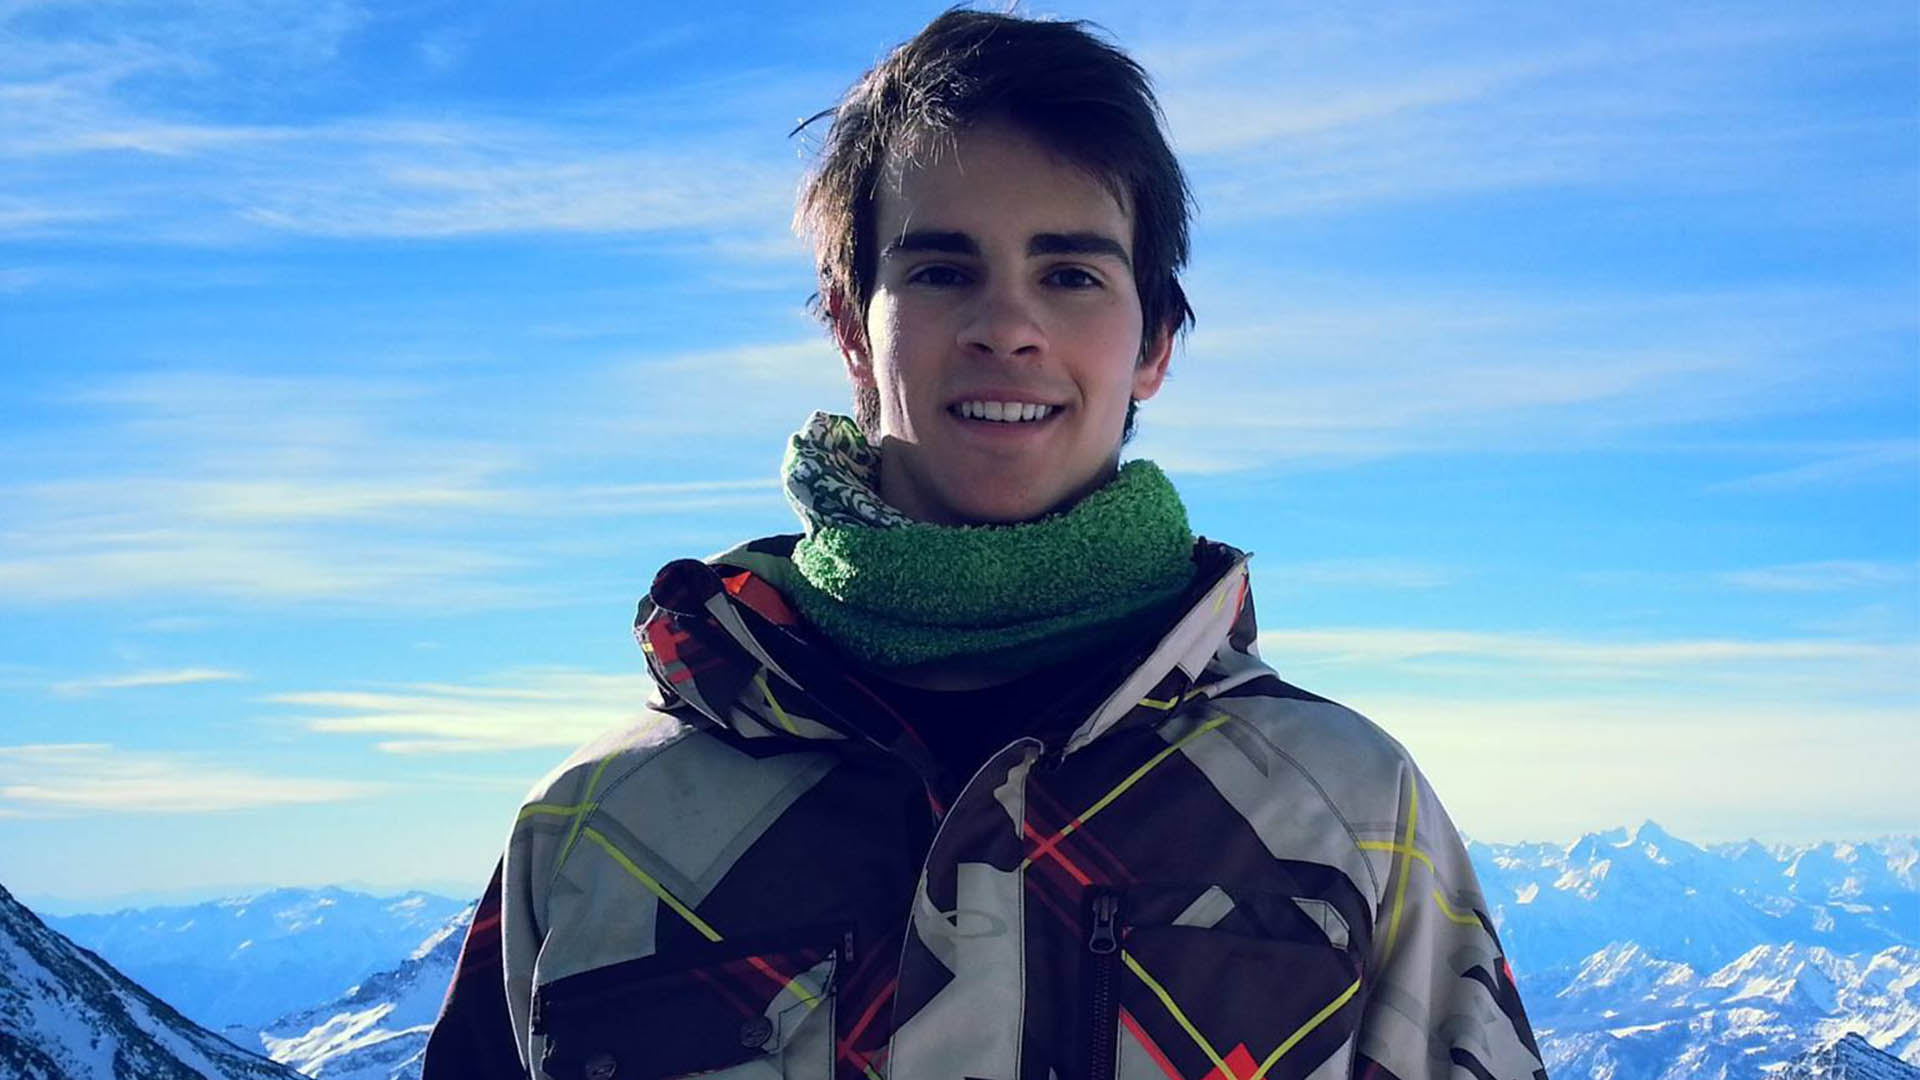
\includegraphics[width=0.7\textwidth]{../dillon.jpg}
			\caption{Dillon Heins}
		\end{figure}
	\subsubsection{Interests}
		\begin{itemize}
			\item Algorithms and data structures
			\item Computer networks
			\item Computer graphics
			\item Computer security
			\item Game development and design
		\end{itemize}
	\subsubsection{Technical Skills}
		\begin{itemize}
			\item Strong programming, algorithmic and data structure skills
			\item Proficient in the use of multimedia i.e. the combining of computer science, visual design and multimedia to create a complete and coherent product
			\item Proficient in the programming and understanding of networked software
			\item Analysis and effective visualisation of information
		\end{itemize}
	\subsubsection{Past Experience \& Achievements}
		\begin{itemize}
			\item \textbf{Past Experience}
			\begin{itemize}
				\item Web Developer for Ms. Vreda Pieterse (Software engineering lecturer)
				\begin{itemize}
					\item University of Pretoria
					\item July 2014 - Present
				\end{itemize}
				\item Teaching Assistant
				\begin{itemize}
					\item University of Pretoria
					\item February 2016 - Present
				\end{itemize}
			\end{itemize}
			
			\item \textbf{Achievements}
			\begin{itemize}
				\item Golden Key member: 2015 - Present
				\item Top achievers' award for BIS Multimedia: 2014 \& 2015
				\item Overall distinction: 2014 \& 2015
				\begin{itemize}
					\item 80.11\% year average: 2015
				\end{itemize}
				\item Dale Carnegie Generation.Next Certificate of Achievement
			\end{itemize}
		\end{itemize}
		
	\subsubsection{Non-technical Skills}
		\begin{itemize}
			\item Diligent and disciplined worker
			\item Strong leader who leads through example and encouragement
			\item Highly motivated and good at motivating others
			\item Communicating effectively and proficiently
			\item Adept in the learning and application of newly acquired skills
			\item Adaptable to change
		\end{itemize}
	\subsubsection{Motivation for Choosing Project}
		This project presents an interesting challenge which would be very satisfying to solve.
		
		Personally I want to do this project as I am fascinated by the intricacies and the workings of networks. By doing this project I feel as though I would learn an immense amount about networks that could only be learnt by doing something as in-depth as this project. This project offers many different sets of problems from the algorithmic and data structure problems to the visualising of the information problems, all of which are problems which I would enjoy solving.
		
		Another main reason for me wanting to do this project is the fact that I enjoy and am skilled in the effective presenting and communicating of information. I feel as though this project offers a great platform to manipulate and visualise very complex information. As a student I too have experienced the problems of not being able to accurately visualise the workings of a network. I believe that given software which would be able to visualise the workings of a network it would assist with the understandings of said networks greatly.
		
		Expanding on the above, this is a project which I would be heavily personally invested in as it offers many rewards for completing it. The software being designed is something which I would personally want to use and being able to create software which one would use is enough motivation in and of itself.

\cleardoublepage
    
\section{Project Execution}

\end{document}
